\section{Errors in the GPS Observables}
	So far the range between a satellite and a receiver has been measured by the pseudorange.A cheap receiver can find this distance with an accuracy of 10 meters. However there are specialized applications of GPS that require accuracies of 1 cm or better. To get to that level of accuracy we must study the signal structure more closely.
	
	The pseudorange is derived from a complicated bookkeeping that tracks the individual chips of the Gold code. Each chip has a length of ca. 300 meters.
	
	Remember the signal combines a carrier wave and a Gold code plus an ephemeris. The latter two are modulo-2 added and modulated on the carrier wave using BFSK.
	
	In 1982 C. C. Counselman III at MIT got the idea to use the carrier wave as measurement unit. So the change in phase of the carrier wave multiplied by the wavelength is an independent estimate of the range, with a resolution comparable to the wavelength (two decimeters). The drawback is that we need to know the integer number N of wavelengths in the range. This number is many millions.
	
	For a crude estimate of N , divide the pseudorange by the wavelength. The more 	precise knowledge of N is left for clever algorithms to reveal. This topic is developed in 	Chapter 10, and we quote (10.7)
	\begin{equation}\label{eq:9.33}
		\Phi^k_i(t) = \rho^k_i-I^k_i+T^k_i+c(dt_i(t)-dt^k(t-\tau^k_i))+\lambda(\varphi_i(t_0)-\varphi^k(t_0)+N^k_i)-\epsilon^k_i
	\end{equation}

	This equation corresponds to (9.19) for the pseudorange observation. A new term$\lambda f=\lambda(\varphi_i(t_0)-\varphi^k(t_0)+N^k_i)$appears in this carrier phase observation.
	
	Note that the sign of the ionospheric delay 1 has changed compared to the equation for the pseudorange. This phenomenon follows from the following argument: The ionosphere is a dispersive medium which means that group and phase delays are different. The group refraction index $n_g$ and the index of refraction for the phase $n_p$ are connected by$n_g=n_p+\partial n_p/\partial f$with $n_p=1-at/f^2=1-I$.Now follows
	\[
		n_g = 1-\dfrac{at}{f^2}+f\dfrac{2at}{f^3}=1+\dfrac{at}{f^2}
	\]
	where a is a constant and t is the number of ionospheric electrons per unit of space. You immediately see that the sign of I is changed from $n_g=1+I$to$n_p=1-I$.
	
	The factor $f=\varphi_i(t_0)-\varphi^k(t_0)+N^k_i$is composed of three terms: the fractional part $\varphi^k$ of the carrier wave at the receiver end, the fractional part $N^k_i$ at the satellite end, and	finally the integer number Nk of waves between satellite and receiver. 
	
	In Chapter 10 we will introduce single and double differences. A single differencing$\Phi^k_i-\Phi^l_i$or$\Phi^k_i-\Phi^k_j$eliminates either $\varphi_i$or$\varphi^k$.But to reach an integer requires differencing once more;we form $\Phi^{kl}_{ij}$.Then the double differenced f equals N.
	
	So a given satellite range can be estimated by a pseudorange $P^k_i$ (less accurate) and	a carrier phase $\Phi^k_i$(more accurate).
	
	One more extension is possible. The GPS signal transmit on both frequencies L1 and L2. So a geodetic receiver observes pseudorange and carrier phase on L1 and L2. That is four observables to find $N_1$ and $N_2$ plus three receiver coordinates and a receiver clock offset. With 10 satellites we have 40 observables and 20 + 4 unknowns.
	
	The fundamental observables are the pseudorange $P^k_i$ and the carrier phase $\Phi^k_i$ between satellite k and receiver i. The phase is much more accurate than the pseudorange (even using the P code). Both observables will include errors from many sources! Some errors can be removed , others can be reduced, and others are just neglected. This section estimates the magnitudes of the errors and our options for dealing with them .
	
	\subsection{Delay of the Signal}
	
		Apart from the receiver and satellite clock errors, the largest errors (until we compensate for them) come from the delay when a signal travels through the atmosphere. So we first recall the connections between velocity and refraction and travel time. Then we estimate the range errors due to incorrect travel times and other sources. We .follow Parkinson $\&$ Spilker Jr. (1996) and Teunissen $\&$ Kleusberg (1998) in estimating the sources of error.
		
		In a vacuum the speed of an electromagnetic wave is c. In the atmosphere, this speed (the phase velocity) is reduced to v.The dimensionless ratio $n=\frac{c}{v}$is the refractive index.The number u is related to the angular frequency $\omega$ and wave bumber k by $v=\frac{\omega}{k}$.
		
		In a dispersive medium, these numbers are functions of $\omega$. A packet of waves with
		frequencies near $\omega$ will travel not with the phase velocity v but with the group velocity:
		\begin{equation}\label{eq:9.34}
			v_{group} = \dfrac{d\omega}{dk}=v+k\dfrac{dv}{dk}
		\end{equation}
		
		That is the travel speed of a modulation superimposed onto the carrier wave. The refractive index becomes$n_{group}=c/v_{group}$.
		
		The wave travels from satellite to receiver along the quickest path S (by Fermat’s principle of least time). At a planar interface in the medium, this principle yields Snell’s law $n_1\sin z_1$ = $n_2\sin z_2$ for the change in the angle z (between the path and the normal to the discontinuity). The delay along S of the carrier, in comparison to the straight-line path L in a vacuum, is $dt_\Phi$ :
		\[
			dt_\Phi = \int_S\dfrac{dS}{v}-\int_L\dfrac{dL}{c}
		\]
		
		Most of this delay comes from change of speed, a smaller part comes from change of path.Multiplying by c, the two parts are
		\begin{equation}\label{eq:9.35}
			c\,dt_\Phi=\int_L(n-1)dL+(\int_Snds-\int_LndL)
		\end{equation}
		
		For the modulation, which carries the important signal for GPS, v becomes ugroup and the refractive index becomes $n_{group}$.
		
		The scientific problem is to determine n and ngroup from properties of the atmosphere, the electron density in the ionosphere and the air/water densities in the troposphere.
	
	\subsection{Error Budget for GPS}
		Here are the principal errors in GPS positioning their sources and also their approximate magnitudes. We estimate errors in the range and multiply by the DOP factors.
		\begin{table}
			\caption{Relative accuracy of clocks}
			\label{tab:9.5}
			\begin{tabularx}{\textwidth}{ll}
				\hline
				Clock type & Relative accuracy \\
				\hline
				Crystal wrist watch & $10^{-6}$ \\
				Geodetic GPS receiver & $10^{-5}-10^{-7}$ \\
				TI, crystal in oven & $10^{-8}-10^{-9}$ \\
				Chip scale atomic clock (CSAC) & $5\times10^{-12}$ \\
				Rubidium & $10^{-11}-10^{-12}$ \\
				Cesium & $10^{-12}-10^{-13}$ \\
				Hydrogen maser & $10^{-15}-10^{-16}$ \\
				\hline
			\end{tabularx}
		\end{table}
		
		\textit{Ephemeris Errors} The satellite transmits its Keplerian elements, almost exactly but with a small error. This grows from the time of upload by a control station until the next upload.The error growth is slow and smooth, and only the projection of the ephemeris error along the line of sight produces an error in the range. Parkinson $\&$ Spilker Jr. (1996) estimate the rms ranging error as 2 meters (and the estimate now might be smaller).
		
		\textit{Satellite Clock Errors} An atomic clock, with a rubidium or cesium oscillator, is correct to about 1 part in $10^{12}$. In a day the offset could reach $10^{-7}$ seconds; multiplied by c this represents 26 meters. With clock corrections every 2 hours, an average 1 meter error in pseudorange is reasonably conservative. Table \ref{tab:9.5} gives a survey of clocks.
		
		\textit{Ionosphere Errors} GPS signals are delayed as they pass through the ionosphere, which starts 50 km above the Earth and extends to 1000 km or more. The delay is proportional to the number of electrons (integrated density along the signal path) and inversely proportional to $f^2$. Thus the effect is dispersive; it depends on the frequency $f$. The density of free electrons varies strongly with the time of day and the latitude. The variations from solar cycles and seasons and especially short-term effects are less strong but less predictable. If the delay were not accounted for at all, the ranging errors on the LI frequency in the zenith direction could reach 30 meters. The effects on the pseudorange P and phase $\Phi$ are opposite in sign; the carrier phase is advanced. 
		
		So we must estimate the ionospheric delay. A dual-frequency receiver can measure the pseudoranges $P_1$ and $P_2$ on both frequencies L1 and L2, and solve for the delay:
		\begin{equation}\label{eq:9.36}
			dP_{ion} = \dfrac{f^2_2}{f^2_2-f^2_1}(P_1-P_2)+random/unmodelled errors.
		\end{equation}
		
		This should be removed from $P_1$. Similarly the phase correction for ionospheric delay is
		\begin{equation}\label{eq:9.37}
			dP_{ion} = \dfrac{f^2_2}{f^2_2-f^2_1}((\lambda_1N_1-\lambda_2N_2)-(\Phi_1-\Phi_2))+random/unmodelled errors.
		\end{equation}
		
		Equations \ref{eq:9.36} and \ref{eq:9.37} have equal value (in delay units) but opposite signs, so the ionosphere can be unambiguously calibrated by a combination of pseudorange and phase at both frequencies.
		
		The ambiguities $N_1$ and $N_2$ remain constant (but possibly unknown) if there are no cycle slips. So at least a differential delay over time is known. This estimate is good but there is often a better way. If you have a dual frequency phase receiver, the P code observations allow you to estimate the ionospheric correction. Then the improved pseudoranges can help resolve the ambiguities $N_1$ and $N_2$, completing the circle.
		
		For measurements at only one frequency, these formulas for $dP_{ion}$ and $d\Phi_{ion}$ are useless. Satellite based augmentation systems offer estimates of $dP_{ion}$ with an accuracy better than 1 m, see Section 9.9.
		
		In DGPS the ionospheric delay at two receivers is canceled when we compute the (sufficiently short!) baseline between them. The difference in signal paths produces a slight baseline shortening, proportional to electron content and baseline length. One receiver at one frequency can use the prediction model for $dP_{ion}$ and $d\Phi_{ion}$ contained in the GPS broadcast message. Tests show better results than promised (but not great).
		
		\textit{Troposphere Errors} The troposphere is the lower part of the atmosphere, thickest over the Equator (about 16 km). The temperature and pressure and humidity alter the speed of radio waves. Their effects are nearly independent of the radio frequency, but they depend on the time of passage. For a flat Earth we would divide the zenith delay (the delay at elevation angle $El=\frac{\pi}{2}$) by sin El. There are a number of good mapping functions to improve this to a spherical-surface model. The M-file tropo uses a mapping function proposed by Goad$\&$Goodman (1974) to compute the reduction.
		
		In the zenith direction, the total tropospheric delay is estimated as about 2.3 meters.The hydrostatic component (responsible for $90\%$) is the path integral of the density of moist air. The wet component is a function of water vapor density which is highly variable.It is questionable how descriptive actual measurements can be. The classical example is sitting in a fog bank only 50 m high. The other extreme is sitting in relatively dry air below a dark thundercloud. Both of these conditions are met in GPS surveys.
		
		In fact Duan et al. (1996) proposed and successfully demonstrated that in the reverse direction, the water vapor density could be measured by GPS! This is a beautiful example of an unexpected contribution coming from accurate measurements of time and distance.
		
		The delay from liquid water in clouds and rain is well below 1 cm. But models of the wet delay (water vapor) using surface meteorology are often wrong by more than 1cm. Again we recommend the discussion by Langley in Teunissen $\&$ Kleusberg (1998).
		
		\textit{Multipath Errors} A GPS signal might follow several paths to a receiver’s antenna. The same signal arrives at different times and interferes with itself. This produces ghost images on TV (before cable) and corresponds to echoes for our voice. In GPS, the signal can be reflected from buildings or the ground and create a range error of several meters or more.Misra $\&$ Enge (2006) allow 5 meters for multipath error in C/A code measurements.
		
		Multipath describes the situation where signals coming from the satellite propagates along several paths to the receiver antenna. The main part of the signal radiates directly from the satellite but part of the signal is reflected from nearby surfaces. Multipath depends on satellite geometry and the antenna environment and this makes multipath difficult to model. For long observation periods 24 hours or more the multipath effects are partly reduced by averaging. However, observation periods most often last only for a few hours or much less; this is why multipath is a problem.
		
		The reflected surfaces shift the phase with respect to the original transmission, and this appears as additive noise at the antenna. Because the antenna locations are different,the multipath signature at each antenna is unique and the error is not common mode.
		
		Multipath is a serious problem because it is so difficult to model. Sometimes we can improve the site for the receiver. The design of the antenna is also critical. Large groundplanes, with various antenna elements (dipoles, microstrip), are the most common antidote for multipath. The receiver can be built with a narrow correlator to block the reflection, or with multiple correlators to allow estimation on several paths. And for a given satellite/static receiver pair, at a given time of day, we could try to estimate repeatable paths. For GPS the satellite geometry repeats every 23 hours and 56 minutes.
		
		The multipath errors in the phase observations are much smaller, at the centimeter level. We analyse the simple situation when a direct signal is superimposed by a reflected signal, with phase shift $\Delta\Phi$ and magnitude attenuated by a factor $\gamma$:
		\begin{align*}
			received signal &= A\cos\Phi+\gamma A\cos(\Phi+\Delta\Phi) \\
								&= A\cos\Phi+\gamma A\cos\Phi\cos\Delta\Phi-\gamma A\sin\Phi\sin\Delta\Phi\\
								&= (A+\gamma A\cos\Delta\Phi)\cos\Phi-(\gamma A\sin\Delta\Phi)\sin\Phi
		\end{align*}
		We now claim that the received signal also can be represented as
		\begin{align*}
			\gamma_MA\cos(\Phi+\Delta\Phi_M) &= \gamma_MA\cos\Phi\cos\Delta\Phi_M-\gamma_MA\sin\Phi\sin\Delta\Phi_M \\
											 &= (\gamma_MA\cos\Delta\Phi)\cos\Phi-(\gamma_MA\sin\Delta\Phi)\sin\Phi
		\end{align*}
		Comparing the coefficients of sin $\Phi$ and cos $\Phi$ we get the following two equations:
		\begin{align*}
			\gamma_M\sin\Delta\Phi_M &=\gamma\sin\Delta\Phi \\
			\gamma_M\cos\Delta\Phi_M &=1+\gamma\cos\Delta\Phi
		\end{align*}
		and their ratio
		\begin{equation*}
			\tan \Delta\Phi_M=\dfrac{\sin\Delta\Phi}{\gamma^{-1}+\cos\Delta\Phi}
		\end{equation*}
		The multipath phase error is
		\begin{equation*}
			\Delta\Phi_M=\arctan(\dfrac{\sin\Delta\Phi}{\gamma^{-1}+\cos\Delta\Phi})
		\end{equation*}
		The worst case has no attenuation (y = 1) and a phase shift $\Delta\Phi_M=90\circ$. This means only a quarter-wavelength error (5 cm) in the phase due to multipath.
		
		Other sources of error exist! Receivers are not perfect but they are continually improving.Of course the Earth is moving up and down (there are tides on dry ground just as in the sea,but smaller). These tides can be accounted for almost completely. The actual position of the Earth’s surface and of sea level affects vertical positioning by GPS, which is less accurate than horizontal positioning. As a limitation on vertical accuracy for precise positioning,tides are less difficult than the troposphere and antenna problems (multipath and phasecenter variations). But still we can land an airplane.
		\begin{table}
			\caption{Standard Errors}
			\centering
			\label{tab:9.6}
			\begin{tabularx}{\textwidth}{lrr}
				\hline
				  & Single frequency & Double frequency \\
				\hline
				Ephemeris data & 2m & 2m \\
				Satellite clock & 2m & 2m \\
				Ionosphere & 4m & 0.5-1m \\
				Troposphere & 0.5-1m & 0.5-1m \\
				Receiver noise and multipath & 0-2m & 0-2m \\
				\hline
				User Equivalent Range Error: rms & 5m & 2-4m \\
				\hline
			\end{tabularx}
		\end{table}
	
	\subsection{easy16}\label{subsec:easy16}
		With a given receiver you get a certain accuracy of your position. The next question may often be: Can I do anything to improve it? The answer most often is: Yes, buy a better receiver! Most ranging errors are determined by physics and you can do little to. improve the accuracy.
		
		Anyway, it is interesting to analyse the information you may get from a single “ oneway,” i.e., a single set of observables $(P_1,\Phi_1,P_2,\Phi_2)$ related to one satellite seen by a dual-frequency receiver. By so doing you also get an insight into the nature of the error sources and which ones do matter and which ones can be modeled or eliminated.
		
		The ephemeris of the tracked satellite yields the elevation angle; the ionospheric delay is estimable for data from a dual-frequency receiver; the tropospheric delay is computed from a standard model; and the remaining errors we call multipath errors. Finally we estimate the orbital errors by comparing satellite positions computed from broadcast and precise ephemerides. The data sample illustrates these different error contributions very well, varying over time and therefore depending on elevation angle.
		
		We select a specific one-way observation set from a station south of Aalborg on January 19, 2007. It is taken from the data set already used in easy15. We select to investigate PRN 14 in the full session length, that is about 42 minutes.
		
		The first subplot in Figure 9.16 depicts the satellite elevation angle which varies from $18\circ$ to $33\circ$. Next one-way errors in ionosphere, troposphere, and multipath are shown.
		
		When dealing with the ionospheric delay I we assume that we have both pseudorange and carrier phase observations on L1 and L2. We estimate the delay / according to the following matrix equation:
		\begin{equation}\label{eq:9.38}
			\begin{bmatrix}
				1 &       1 &         0 & 0 \\
				1 &      -1 & \lambda_1 & 0 \\
				1 &  \alpha & 		  0 & 0 \\
				1 & -\aleph & 		  0 & \lambda_2
			\end{bmatrix}
			\begin{bmatrix}
				\rho^* \\ I \\ N_1 \\ N_2
			\end{bmatrix}=
			\begin{bmatrix}
				P_1 \\ \Phi_1 \\ P_2 \\ \Phi_2
			\end{bmatrix}+e
		\end{equation}
		
		As usual $\alpha=(f_1/f_2)^2=I_2/I_1$
		
		\begin{figure}
			\centering
			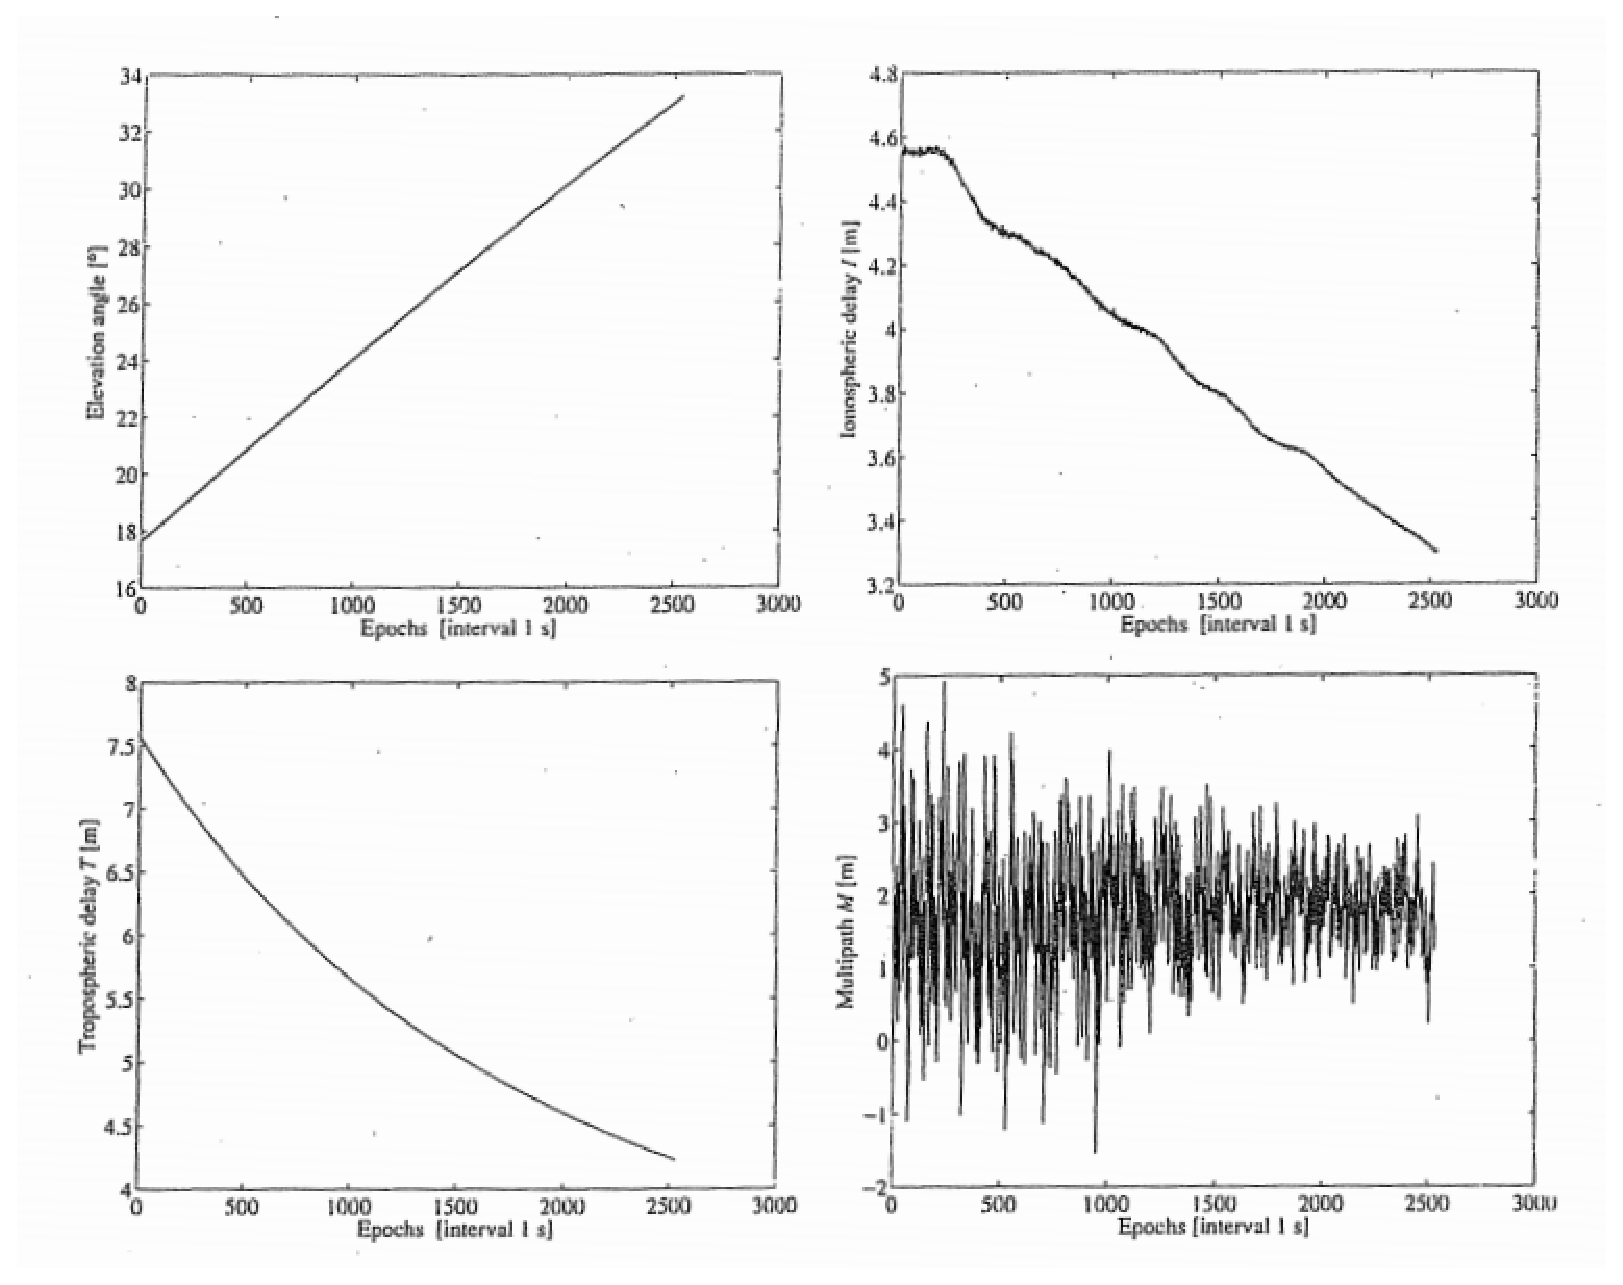
\includegraphics[width=0.7\linewidth]{TeX_files/Part03/chapter09/image/9-16}
			\caption{Angle and one-way errors: Ionosphere, troposphere, multipath.}
			\label{fig:9-16}
		\end{figure}
		First we estimate $N_1$ and $N_2$as reals; incorrect values for $N_1$ and $N_2$just change the level for I.Next we estimate I alone as
		\begin{equation}\label{eq:9.39}
			I=\dfrac{-\lambda_1N_1+\lambda_2N_2+\Phi_1-\Phi_2}{\alpha-1}
		\end{equation}
		
		For the tropospheric delay we use the Goad-Goodman model. The delay T ranges from 7.4 m to 4.2 m. If the satellite passed zenith, T would have been about 2.5 m
		Let the geometrical distance between satellite and receiver be $\rho$, let I be the ionospheric delay, and M the multipath including receiver noise. The pseudoranges observed on L1 and L2 may then be expressed as
		\begin{align}\label{eq:9.40}
			P_1&=\rho+I_1+M_1 \\
			P_2&=\rho+I_2+M_2 
		\end{align}\label{eq:9.41}
		Remaining errors are identified as multipath and receiver noise.
		
		Similarly for the phase observations
		\begin{align}\label{eq:9.42}
			\Phi_1&=\rho-I_1+\lambda_1N_1+m_1=\lambda_1\varphi_1 \\
			\Phi_2&=\rho-I_2+\lambda_2N_2+m_2=\lambda_2\varphi_2 
		\end{align}\label{eq:9.43}
		\begin{figure}
			\centering
			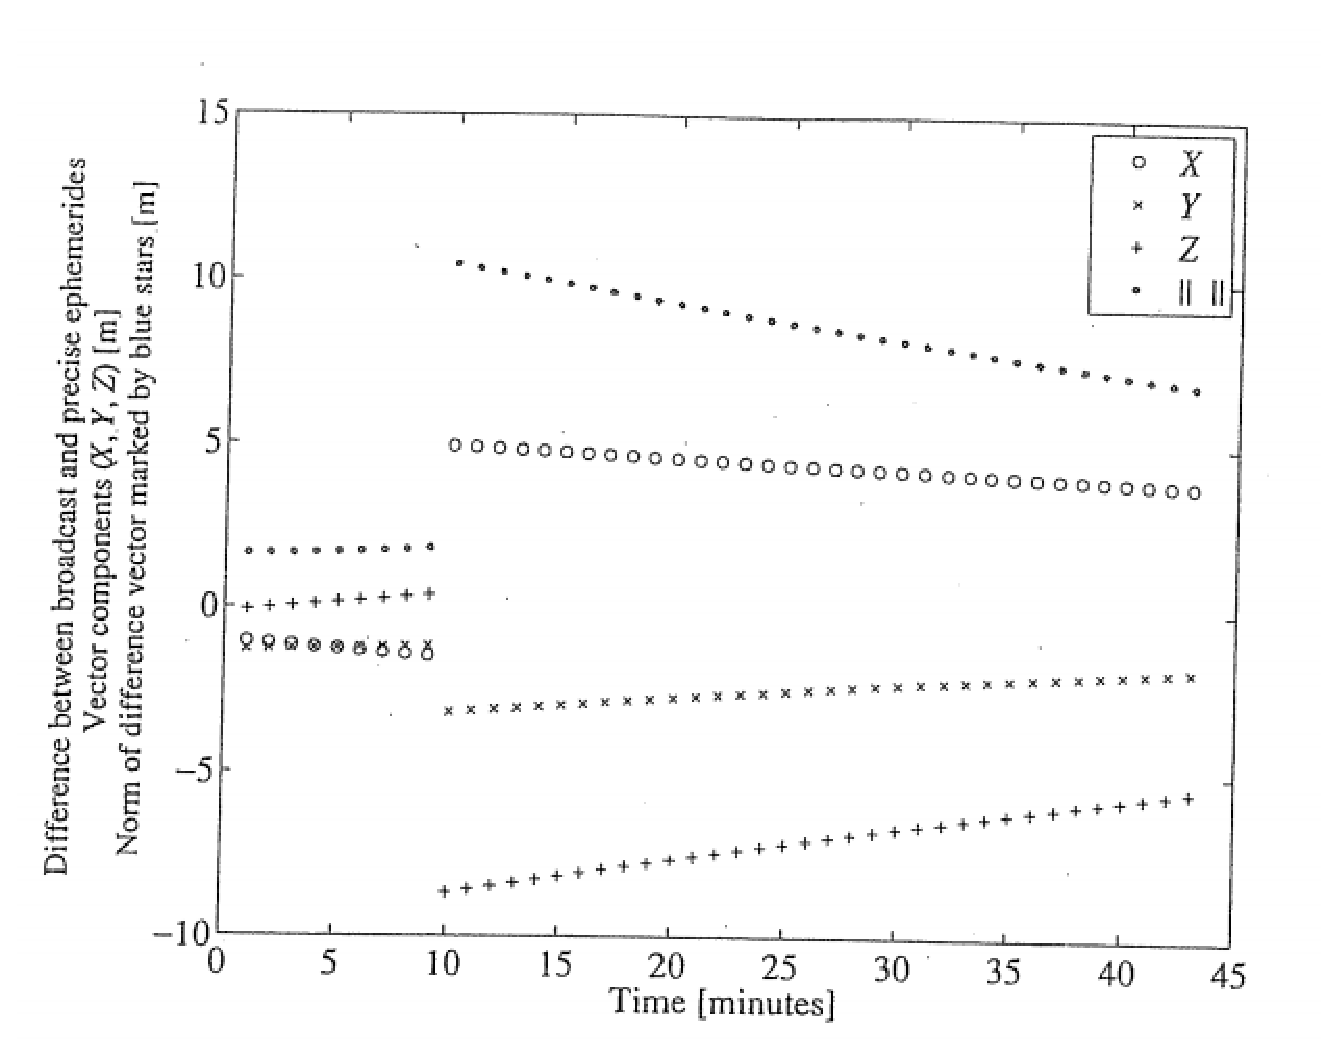
\includegraphics[width=0.7\linewidth]{TeX_files/Part03/chapter09/image/9-17}
			\caption{Difference between precise and broadcast ephemerides}
			\label{fig:9-17}
		\end{figure}
		The multipath on phase observations is so small that we subsequently put $m_i = 0$. We
		want to find an expression for $M_1$ . We start by subtracting \ref{eq:9.42} from \ref{eq:9.40}:
		\begin{equation*}
			P_1-\Phi_1=2I_1+M_1-\lambda_1N_1
		\end{equation*}
		or
		\begin{equation}\label{eq:9.44}
			M_1-\lambda_1N_1=P_1-\Phi_1-2I_1
		\end{equation}
		and subtracting \ref{eq:9.43}from\ref{eq:9.42}yields
		\begin{equation}\label{eq:9.45}
			\Phi_1-\Phi_2=I_2-I1+\lambda_1N_1-\lambda_2N_2=(\alpha-1)I_1+\lambda_1N_1-\lambda_2N_2
		\end{equation}
		or
		\begin{equation}\label{eq:9.46}
			I_1=\dfrac{1}{\alpha-1}(\Phi_1-\Phi_2)+\dfrac{1}{\alpha-1}(\lambda_2N_2-\lambda_1N_1)
		\end{equation}
		We insert \ref{eq:9.46}into\ref{eq:9.44}and obtain
		\begin{equation}\label{eq:9.47}
			M_1-\lambda_1N_1=P_1-\Phi_1-\dfrac{2}{\aleph-1}(\Phi_1-\Phi_2)-\dfrac{2}{\alpha-1}(\lambda_2N_2-\lambda_1N_1)
		\end{equation}
		or
		\begin{equation}\label{eq:9.48}
			M_1-(\lambda_1N_1-\dfrac{2}{\alpha-1}(\lambda_2N_2-\lambda_1N_1))=P_1-(\dfrac{2}{\aleph-1}+1)\Phi_1+\dfrac{2}{\aleph-1}\Phi_2
		\end{equation}
		It is reasonable to assume $E\{M_1\} = 0$. The second term on the left side of \ref{eq:9.48} is a constant so it is possible to reduce $M_1$ to $M^*_1$ such that $E\{M^*_1\} = 0$:
		\begin{equation}\label{eq:9.49}
			M^*_1=P_1-\dfrac{\alpha+1}{\alpha-1}\Phi_1+\dfrac{2}{\alpha-1}\Phi_2
		\end{equation}
		Analogously, by exchanging subscripts, we have for the pseudorange multipath on L2:
		\begin{equation}\label{eq:9.50}
			M^*_2=P_2-\dfrac{\alpha+1}{\alpha-1}\Phi_2+\dfrac{2\alpha}{\alpha-1}\Phi_1
		\end{equation}
		
		For all epochs with all four observations $P_1$,$P_2$,$\Phi_1$,and $\Phi_2$ available, we compute multipath according to \ref{eq:9.49}. In the present case, on average the error is below 2m and more noisy for low satellite elevation angles, The noisy character of the plot reflects the actual noise in any pseudorange observation.
		
		Finally we investigate the difference between precise and broadcast ephemerides.
		
		Any file containing broadcast ephemerides is specific to the site where the satellites were tracked. Therefore we need to identify the tracked satellites in the time period where we want to compare the precise and broadcast ephemerides. This can be done by inspecting the corresponding observation file and getting the date and the seconds of week; next we find the corresponding Julian Day Number jd. We find an epoch (modulo 15 minutes) 60 minutes ahead of jd. jd is counted in unit of day. Finally the GPS week number is computed.
		
		Precise ephemerides can be found at igscb.jpl.nasa.gov/igscb/product/1410. Here 1410 is the GPS week number. The file extracts to igr14105.sp3 which contains precise ephemerides for 17 January 2007 in the SP3 format. The IGS SP3 files typically contain satellite positions (X,Y,Z) and clock offsets for each satellite every 15 minutes, from 0:00 hours to 23:45. The SP3 file starts with some header lines which we skip.
		
		We read precise orbits for the interpolation period plus three times 15 minutes ahead and 15 minutes after the period, i.e. 13:15 hours, 13:30 hours, ..., 15:15 hours, in total 9 sets. The precise coordinates for all tracked satellites are stored in Xp.
		
		In the following we introduce a time scale in unit of 15 minutes. This could as well be chosen as whole minutes. The first observation is from 13.85 hours, and the last observation is taken at 14.55 hours. The entire observation period is 2 535 seconds = 42.25 minutes = 2.8 quarters of an hour.
		\begin{figure}
			\centering
			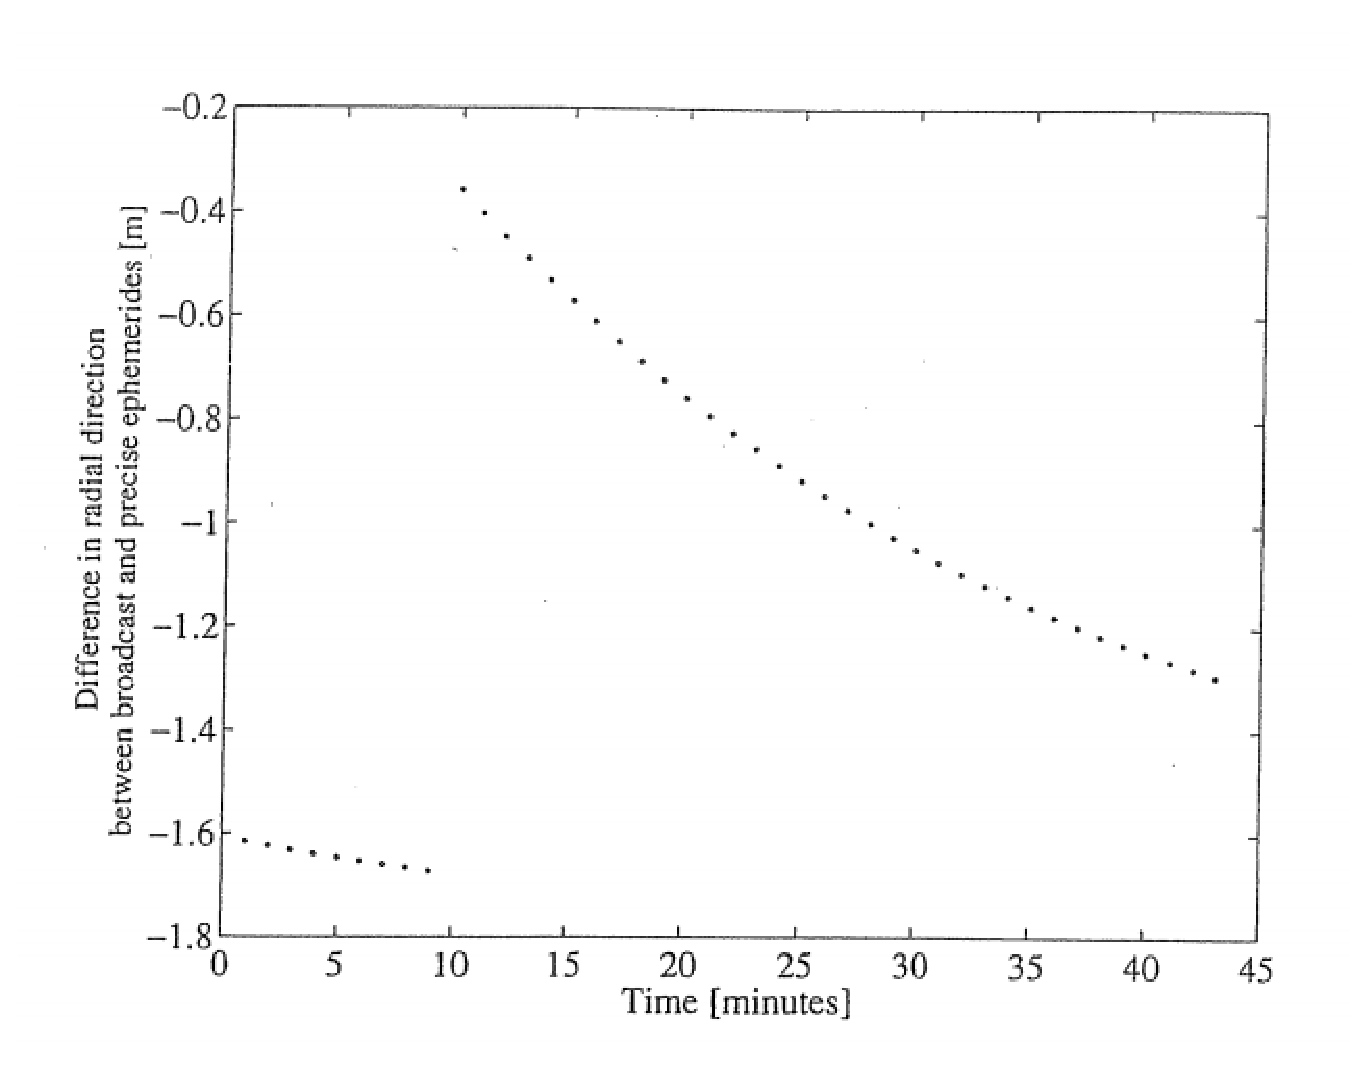
\includegraphics[width=0.7\linewidth]{TeX_files/Part03/chapter09/image/9-18}
			\caption{Length of difference vector between precise and broadcast ephemerides, as projected onto the line of sight.}
			\label{fig:9-18}
		\end{figure}
		
		A Lagrange interpolation for each coordinate, of at least 7th order, is used to compute the actual position. We want an interpolated position each minute, hence we divide by 15 to keep units in quarters of an hour. The first parameter in the i n t p procedure describes the time at which we know the satellite coordinates. The second parameter contains these coordinates, and the third parameter describes the point set at which we want interpolated values, all in units of quarter of an hour. Each coordinate is interpolated separately!
		
		Figure \ref{fig:9-18} shows the difference in satellite position as computed from broadcast ephemerides given via the navigation file, and the post-processed satellite positions for PRN 14. When comparing with broadcast ephemerides we assume the precise positions as the true ones.
		
		The actual influence of the orbit error on the receiver position is given by the projection of the difference vector onto the line between receiver and satellite. Let b be the difference vector between the satellite positions computed from the broadcast and the precise ephemerides. Let a be the vector between the receiver and the satellite position as computed from broadcast ephemerides. Then the projection p of b onto a is
		\begin{equation*}
			p=\dfrac{a^Tb}{a^Ta}a
		\end{equation*}
		
		Figure \ref{fig:9-18} shows this vector p for PRN 14. The computed epherneris error varies in the range of $\pm2m$. The discontinuities reflect epherneris updates at 2-hour intervals.
		
	\subsection{easy10}\label{subsec:easy10}
		For a dual-frequency receiver we can estimate the ionospheric delay Ik by \ref{eq:9.39} or \ref{eq:9.46}:
		\begin{equation*}
		I_k=\dfrac{(\Phi_{2,k}-\Phi_{1,k})-(\lambda_2N_2-\lambda_1N_1)}{1-\alpha}
		\end{equation*}
		We are only interested in changes of $I_k$ over time for the individual PRNs, so we may omit the last, constant term. This leaves the simple expression for the ionospheric delay
		\begin{equation*}
		I_k=(\Phi_{2,k}-\Phi_{1,k})/(1-\alpha)
		\end{equation*}
		Estimates of h for the various PRNs are shown in Figure \ref{fig:9-19}. The data are from file kofil.01o, is to be compared with the upper right part of Figure 9.16 for one PRN.
		\begin{figure}
			\centering
			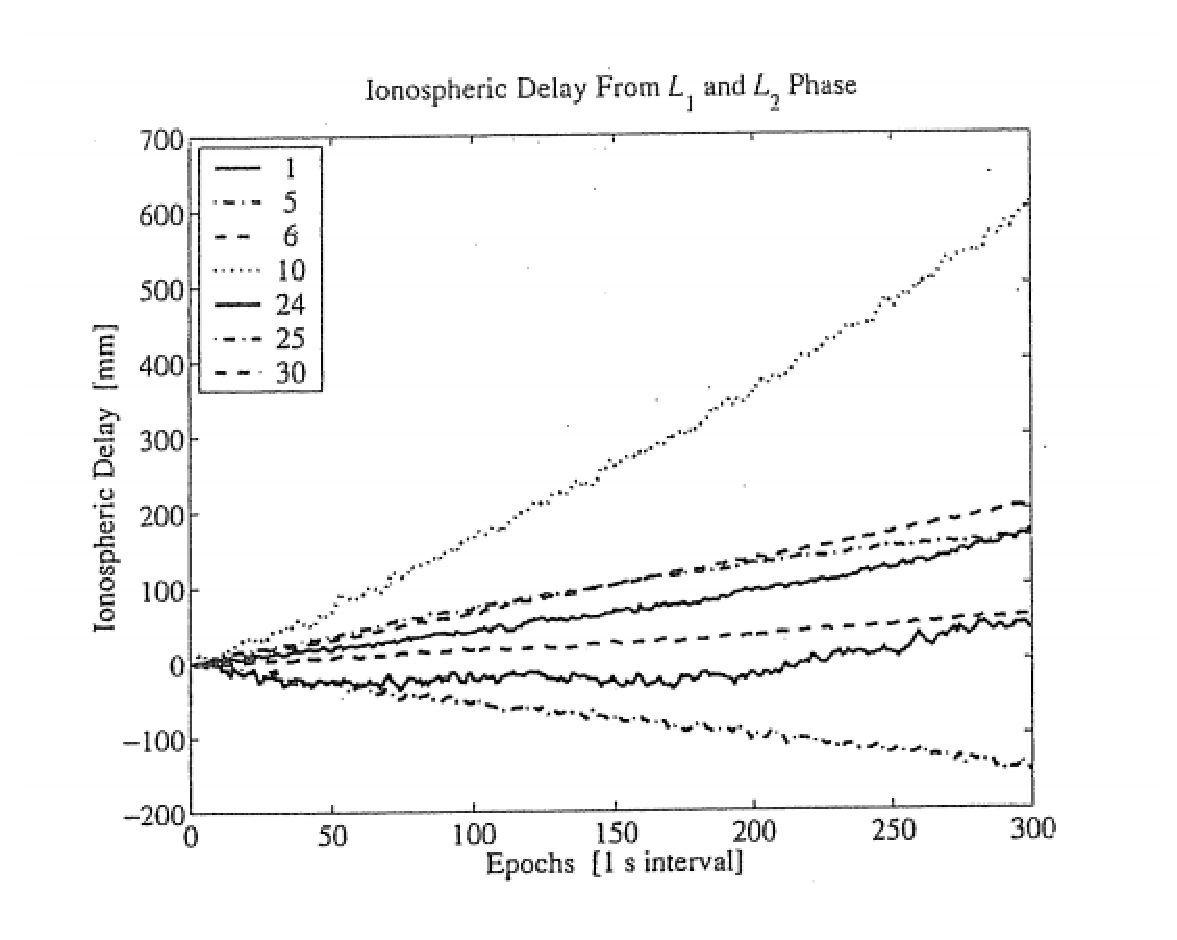
\includegraphics[width=0.7\linewidth]{TeX_files/Part03/chapter09/image/9-19}
			\caption{Ionospheric delay as a function of time}
			\label{fig:9-19}
		\end{figure}
	
	\subsection{Summary of the Error Budget}
	Table \ref{tab:9.6} gives approximate rms errors. The error sources are reasonably independent, so the square root of sum of squares is the UERE the user equivalent range error. This is multiplied by the Dilution of Precision (say VDOP = 2.5 and HDOP = 2) to give the standard deviation in position— in other words, the one sigma error.
	
	This overall range error multiplied by the DOP factor in Section 9.5 is roughly 10 meters for a single frequency  civilian C/A receiver. A dual-frequency P/Y code receiver would experience roughly half that error, when ionospheric delay is cancelled and the ephemeris and clock errors become the largest. Elsewhere we discuss the double differences and longtime averages and carrier phase observations and Kalman filtering that reduce the position error to centimeters and even millimeters.
	
	In the next section we demonstrate how exterior information on ionospheric delay can improve the single point position to a standard deviation of 1 m or better.
